%%%%%%%%%%%%%%%%%%%%%%%%%%%%%%%%%%%%%%%%%%%%%%%%%%%%%%%%%%%%%%%%%%%%%%%%%%%%%%%
% CAPÍTULO 4 - PROPUESTA DE DISEÑO DEL SITIO WEB DEL PROYECTO
%%%%%%%%%%%%%%%%%%%%%%%%%%%%%%%%%%%%%%%%%%%%%%%%%%%%%%%%%%%%%%%%%%%%%%%%%%%%%%%
\chapter{Propuesta de diseño del sitio web del proyecto}
\label{chap:webProp}
Tras la gestión necesaria que necesita un paquete de software desarrollado en Python. En el presente capítulo se muestra la solución web para el software desarrollado de PyCardio, donde trataremos de mostrar las partes que la componen y como han sido implementadas.

Para mostrar la web, el proceso que seguirá esta memoria es la de ir sección por sección donde enseñamos tanto el resultado como la implementación que sigue.

Antes de comenzar, debemos destacar que dicha web se ha implementado utilizando una plantilla adquirida por el equipo de la universidad y diseñada por el equipo WrapBootstrap, esta plantilla se la conoce en dicho servicio como Unify. 

%%%%%%%%%%%%%%%%%%%%%%%%%%%%%%%%%%%%%%%%%%%%%%%%%%%%%%%%%%%%%%%%%%%%%%%%%%%%%%%%%%%%%%%%%%
%                       HOME
%%%%%%%%%%%%%%%%%%%%%%%%%%%%%%%%%%%%%%%%%%%%%%%%%%%%%%%%%%%%%%%%%%%%%%%%%%%%%%%%%%%%%%%%%%
\section{Home}
\label{sec:homeWeb}
Nada más acceder en la web de PyCardio, nos encontramos en el home de la página. El Home se ha implementado de manera que sea lo más visual y sencillo para el usuario, de modo que nada más entrar se nos ofrece la interfaz de todas las secciones, una breve descripción de qué es PyCardio, y los enlaces para redirigirnos a la documentación alojada en Read The Docs, y al código de software a la última release alojada en GitHub. 

\begin{figure}[H]
    \centering
    \subfloat[Home 1]{
        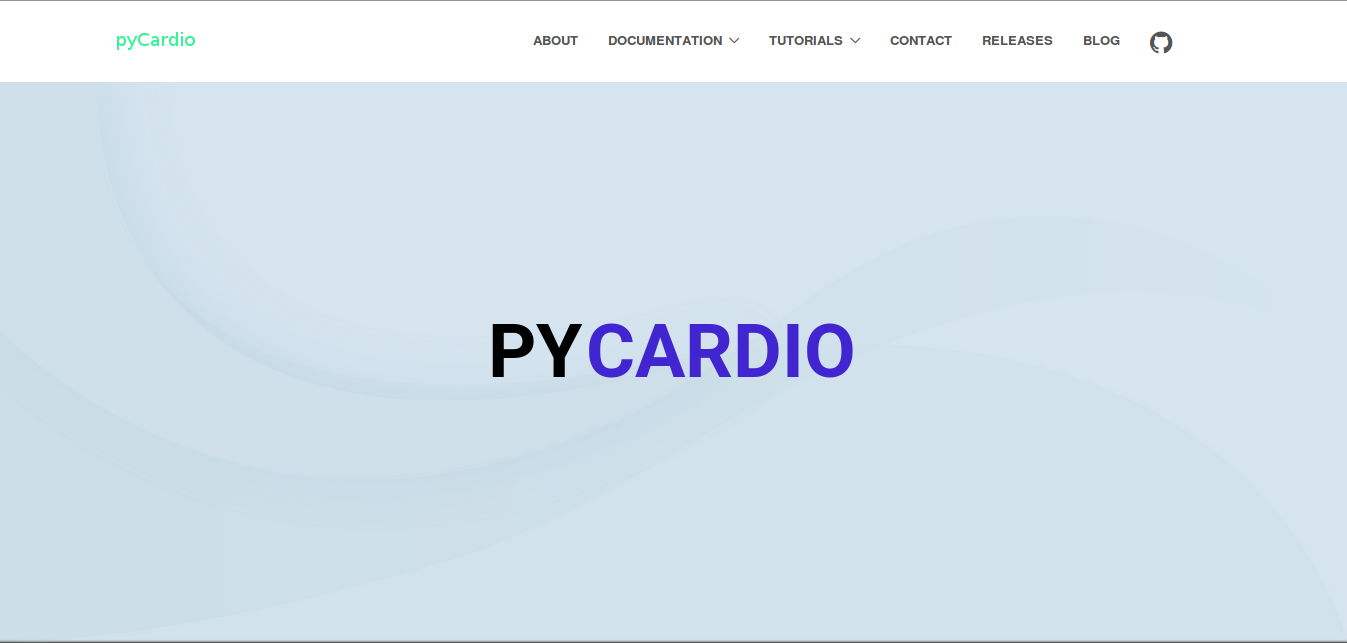
\includegraphics[width=0.3\textwidth]{img/home_1.png}
        \label{fig:home1}
        }
    \subfloat[Home 2]{
        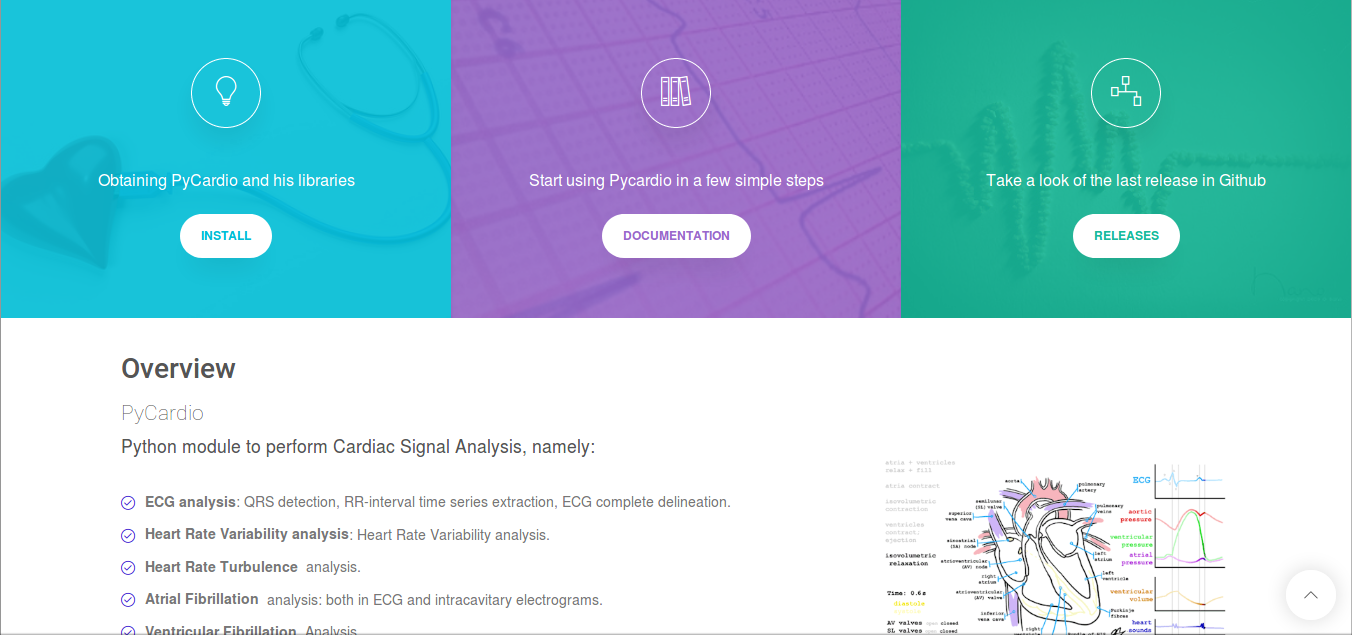
\includegraphics[width=0.3\textwidth]{img/home_2.png}
        \label{fig:home2}
    }
    \subfloat[Home 3]{
        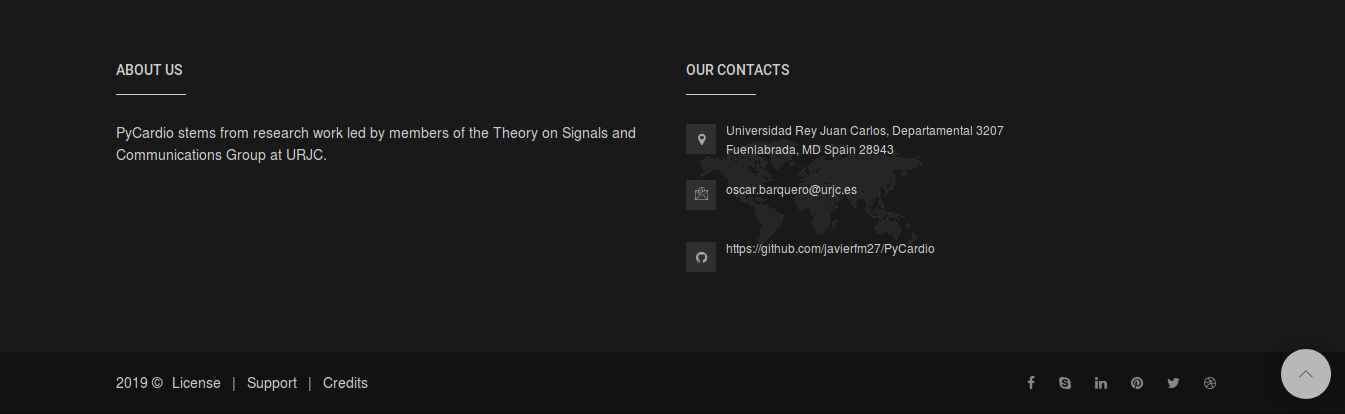
\includegraphics[width=0.3\textwidth]{img/home_3.png}
        \label{fig:home3}
    }
    \caption{Home de PyCardio}
    \label{fig:homePyCardio}
\end{figure}

Para su implementación, lo primero que se realiza es la creación de un fichero \texttt{index} en la raíz del proyecto, donde Jekyll interpretará que dicho fichero será el HTML principal de la web. El fichero puede ser escrito como ya se ha comentado, en MarkDown o en lenguaje de marcado HTML, en nuestro caso, MarkDown. El fichero solo se compone de un Front Matter en el que se llama al layout de Main, y a su vez proporciona el título de la página principal.
\begin{lstlisting}[language=yaml,caption=index.md. Fichero de home de PyCardio,label=co]
    ---
layout: main
title: PyCardio Home
    ---
\end{lstlisting}

El contenido del layout main se compondrá de lenguaje HTML. Este contenido además se rellena con los mencionados \textbf{includes} en el \ref{subsec:githubJekyll}, que compondrán aquel código que se repetirá en todas las secciones de la web, permitiendo así centralizar el desarrollo de manera que, si quisiéramos cambiar el contenido de estos componentes solo tendríamos que realizar dicho cambio en un solo fichero. Para el desarrollo de este prototipo web, se han distinguido los siguientes:
\begin{itemize}
    \item \textbf{\texttt{css.html}}: En él, se incluyen todos los enlaces a los archivos CSS necesarios para la presentación final de la web.
    \item \textbf{\texttt{js.html}}: Incluye los enlaces a los archivos necesarios para el contenido de la web que hace uso de JavaScript.
    \item \textbf{\texttt{header.html}}: Contiene el panel de navegación de todas las secciones de la web.
    \item \textbf{\texttt{footer.html}}: Parte final de todas las páginas que componen la web. En ella se incluye la licencia bajo la cuál está el software, enlaces a las redes sociales del proyecto, y enlace a soporte.
    \item \textbf{\texttt{breadc.html}}: Compone el camino en el que nos encontramos dentro de la web. En él, hacemos uso del lenguaje Liquid para poder construir dicho contenido. 
\end{itemize}

Si observamos las imágenes de la figura \ref{fig:homePyCardio} podemos ver que en el layout referenciado (\texttt{ main.html})  tendremos los includes de \texttt{footer.html} y \texttt{header.html}, además de los de CSS y Javascript, estos procurarán ir en todas las páginas de la web. 

\begin{figure}[H]
    \centering
    \subfloat[header]{
        
\includegraphics[width=0.3\textwidth]{img/header.png}
        \label{fig:includHeader}
        }
    \subfloat[breadcrumber]{
        
\includegraphics[width=0.3\textwidth]{img/breadc.png}
        \label{fig:includBread}
    }
    \subfloat[footer]{
        
\includegraphics[width=0.3\textwidth]{img/footer.png}
        \label{fig:includFooter}
    }
    \caption{Includes de PyCardio}
    \label{fig:includ}
\end{figure}

Así, el Home de la web al ser una página única que no va a tener parecido alguno en lo restante de web excepto en los \texttt{includes} mencionados, el propio layout main, es la página desarrollada, por esto \texttt{index.md} solo se compone de la llamada a dicha plantilla y del título. 

Antes de pasar a tratar la siguiente sección de la web, cabe mencionar que se crea un \texttt{include} más denonminado \texttt{script.html}, donde irá al final de los layouts desarrollados que contendrán aquella tecnología JQuery y Javascript que utiliza la plantilla para hacer de la web   ``sensible'', o como llamamos hoy  día a este tipo de webs \textit{responsive}.
%%%%%%%%%%%%%%%%%%%%%%%%%%%%%%%%%%%%%%%%%%%%%%%%%%%%%%%%%%%%%%%%%%%%%%%%%%%%%%%%%%%%%%%%%%
%                       ABOUT
%%%%%%%%%%%%%%%%%%%%%%%%%%%%%%%%%%%%%%%%%%%%%%%%%%%%%%%%%%%%%%%%%%%%%%%%%%%%%%%%%%%%%%%%%%
\section{About}
\label{sec:aboutWeb}
Esta sección de la web trata de dar una vista general de todos aquellos que han formado parte del proyecto PyCardio, tanto para su parte de desarrollo de software como en la parte de implementación de la web. 

\begin{figure}[H]
    \centering
    \subfloat[About 1]{
        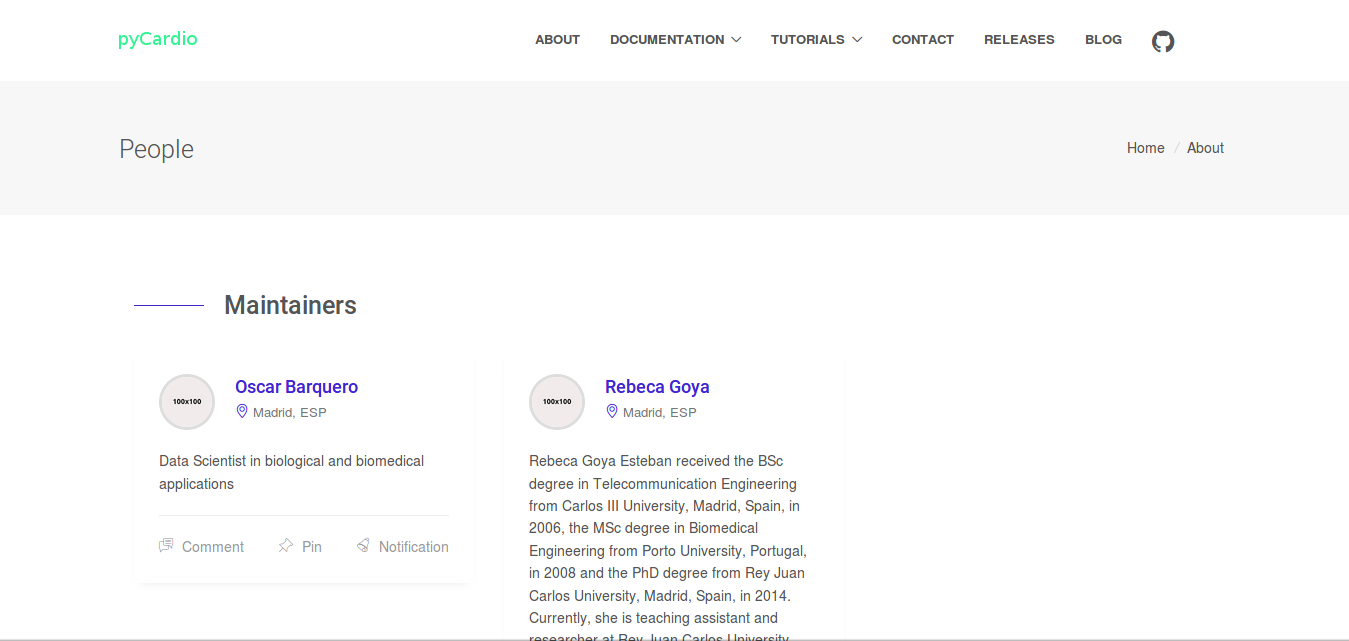
\includegraphics[width=0.5\textwidth]{img/about_1.png}
        \label{fig:aboutWeb1}
    }
    \subfloat[About 2]{
        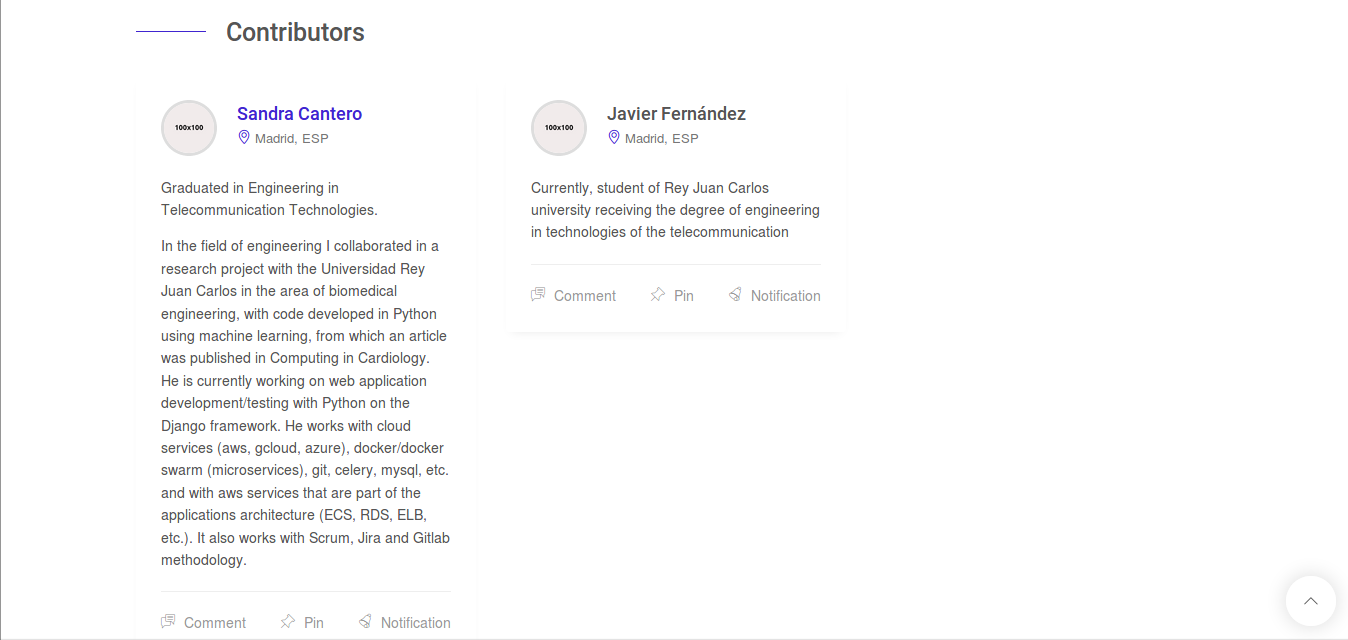
\includegraphics[width=0.5\textwidth]{img/about_2.png}
        \label{fig:aboutWeb2}
    }
    \caption{Sección About de la web PyCardio}
    \label{fig:aboutWeb}
\end{figure}

Para llevar a cabo esta sección, se ha diseñado un nuevo layout denominado \texttt{page.html} cuyo código es mostrado en el listing \ref{code:layoutPage}, que será utilizado para la mayoría de las páginas que se quieran añadir a la web. Tanto Jekyll en su documentación como nosotros, hacemos la siguiente distinción entre estos dos tipos de páginas:

\begin{itemize}
    \item \textbf{Pages: } Contenido que no está basado en una fecha.
    \item \textbf{Posts: } Aquel contenido que se caracteriza por la fecha en la que se publicó en la web.
\end{itemize}

\begin{lstlisting}[style=htmlcssjs,caption=Layout Page,label={code:layoutPage}]
<!DOCTYPE html>
<html lang="en">
<head>
  <!-- Title -->
  <title>{{page.title}} | PyCardio</title>

  <!-- Required Meta Tags Always Come First -->
  <meta charset="utf-8">
  <meta name="viewport" content="width=device-width, initial-scale=1, shrink-to-fit=no">
  <meta http-equiv="x-ua-compatible" content="ie=edge">

  <!-- Google Fonts -->
  <link href="https://fonts.googleapis.com/css?family=Open+Sans:300,400,600,700,800" rel="stylesheet">

  
  <meta http-equiv="refresh" content="5; url=/">
  


  
  

</head>

<body>
  
  
  

  <div class="container g-mt-50 g-mb-60">
    {{ content }}
  </div>

  

  
</body>
\end{lstlisting}

Si observamos la plantilla mencionada, percibimos que para el desarrollo de \textit{About} usamos una variable nueva dónde el contenido se incrustará en  dicha variable del lenguaje de plantilla Liquid denominada \texttt{content}. Al incluir \textit{shortcodes}\footnote{Fragmentos de código utilizadas por los plugins que en este caso se adjuntan con la plantilla Unify adquirida.} de la plantilla Unify el contenido que tendrá nuestro fichero principal de la sección \textit{about} será HTML.

El \textit{shortcode} empleado trata de un elemento de bloque en el que solo se hace uso de los CSS en conjucción con la plantilla. Quedando así tal y como lo muestra el listing \ref{code:about}. 
\begin{lstlisting}[style=htmlcssjs,caption=index.html de About,label={code:about}]
---
layout: page
title: People
---
<div class="container">
  <br>
  <!-- HEADING  MAINTAINERS-->
  <div class="shortcode-html">
    <div class="u-heading-v6-2 g-mb-20">
      <h2 class="h3 u-heading-v6__title g-brd-primary">Maintainers</h2>
    </div>
  </div>
  <!-- END HEADING MAINTAINERS-->

  <!-- TEAM BLOCK -->
  <div class="row">
    <div class="col-lg-4 g-mb-30">
      <!-- Figure -->
      <figure class="u-shadow-v19 g-bg-white g-rounded-4 g-pa-25">
        <div class="media g-mb-20">
          <div class="d-flex g-mr-20">
            <!-- Figure Image -->
            <div class="g-brd-around g-brd-3 g-brd-gray-light-v3 rounded-circle">
              <img class="rounded-circle g-width-50 g-height-50" src="../../assets/img-temp/100x100/img7.jpg" alt="Image Description">
            </div>
            <!-- Figure Image -->
          </div>
          <div class="media-body">
            <!-- Figure Info -->
            <h4 class="h5 g-mb-2"><a href="https://gestion2.urjc.es/pdi/ver/oscar.barquero#tab_1_5">Oscar Barquero</a></h4>
            <div class="d-block">
              <i class="g-color-primary g-font-size-default icon-location-pin"></i>
              <span class="g-color-gray-dark-v4 g-font-size-13">Madrid, ESP</span>
            </div>
            <!-- End Figure Info -->
          </div>
        </div>

        <p>Data Scientist in biological and biomedical applications</p>
      </figure>
      <!-- End Figure -->
    </div>
\end{lstlisting}

Antes de continuar probablemente os hayáis preguntado el porqué de otro fichero \texttt{index} si ya habíamos diseñado uno para el \texttt{home} de nuestra web. Pues bien,  cuando tenemos varias páginas en nuestra página web, lo más eficaz es seguir un orden en los directorios. Por lo tanto si estamos desarrollando la sección \texttt{about}, tengamos en un directorio \texttt{/about/}, todos aquellos contenidos que compondrán esta sección. De manera que, para Jekyll, el fichero en el directorio \texttt{/about/index.html}, será el fichero principal para esa sección.

Así si escribimos un hiperenlace en nuestro web escribiendo \texttt{\{\{site.url\}\}/about/} \footnote{\texttt{\{\{site.url\}\}} es una variable del \textit{framework} Jekyll definido en el fichero de configuración(\texttt{config.yml}) donde obtenemos la dirección URL del sitio web}, nos mostrará el contenido generado por \texttt{index.html} en nuestro directorio \texttt{/about/}.

Cabe destacar la introducción de un nuevo elemento en el \textit{layout} del que se hace referencia en esta sección, haciendo uso del \textit{include} de \texttt{breadc.html} y utilizando la variable \texttt{page}, que brinda información de página específico, permitiendo el uso de las variables definidas en el Front Matter, y de setencias de control del lenguaje de plantilla Liquid,  diferenciándole del mencionado con anterioridad. 

\begin{lstlisting}[style=htmlcssjs,caption=Breadcrumber,label={code:breadcrum}]
  <div class="align-self-center ml-auto">
          <ul class="u-list-inline">
            <li class="list-inline-item g-mr-5">
              <a class="u-link-v5 g-color-main" href="{{site.url}}">Home</a>
              <i class="g-color-gray-light-v2 g-ml-5">/</i>
            </li>
            
            
            

               
                
                  <li class="list-inline-item g-mr-5">
                  {{page.title}}
                  </li>
                
              
                <li class="list-inline-item g-mr-5">
                  <a class="u-link-v5 g-color-main">{{ element |capitalize }}</a>
                  

                  
                    <i class="g-color-gray-light-v2 g-ml-5">/</i>
                  
                </li>
              

            
          </ul>
        </div>
\end{lstlisting}

En este caso el uso que hacemos de la información es el dado por \texttt{\{\{page.path\}\}} y de \texttt{\{\{page.title\}\}} donde accedemos al directorio y título del archivo que hace uso de en este caso, de \texttt{breadc.html}.

%%%%%%%%%%%%%%%%%%%%%%%%%%%%%%%%%%%%%%%%%%%%%%%%%%%%%%%%%%%%%%%%%%%%%%%%%%%%%%%%%%%%%%%%%%
%                       DOCUMENTATION
%%%%%%%%%%%%%%%%%%%%%%%%%%%%%%%%%%%%%%%%%%%%%%%%%%%%%%%%%%%%%%%%%%%%%%%%%%%%%%%%%%%%%%%%%%
\section{Documentation}
\label{sec:docWeb}

Apartado donde se da a conocer el software desarrollado, para ello esta sección se divide en dos, donde por una parte se trata el paquete con una perspectiva general de su utilidad, de lo que trata y de los módulos que lo componen y por otro lado se da a conocer de todas las funciones que componen PyCardio, es decir, la documentación de funciones, módulos, y clases del software.

\begin{figure}[H]
    \centering
    \subfloat[Sección Overview]{
        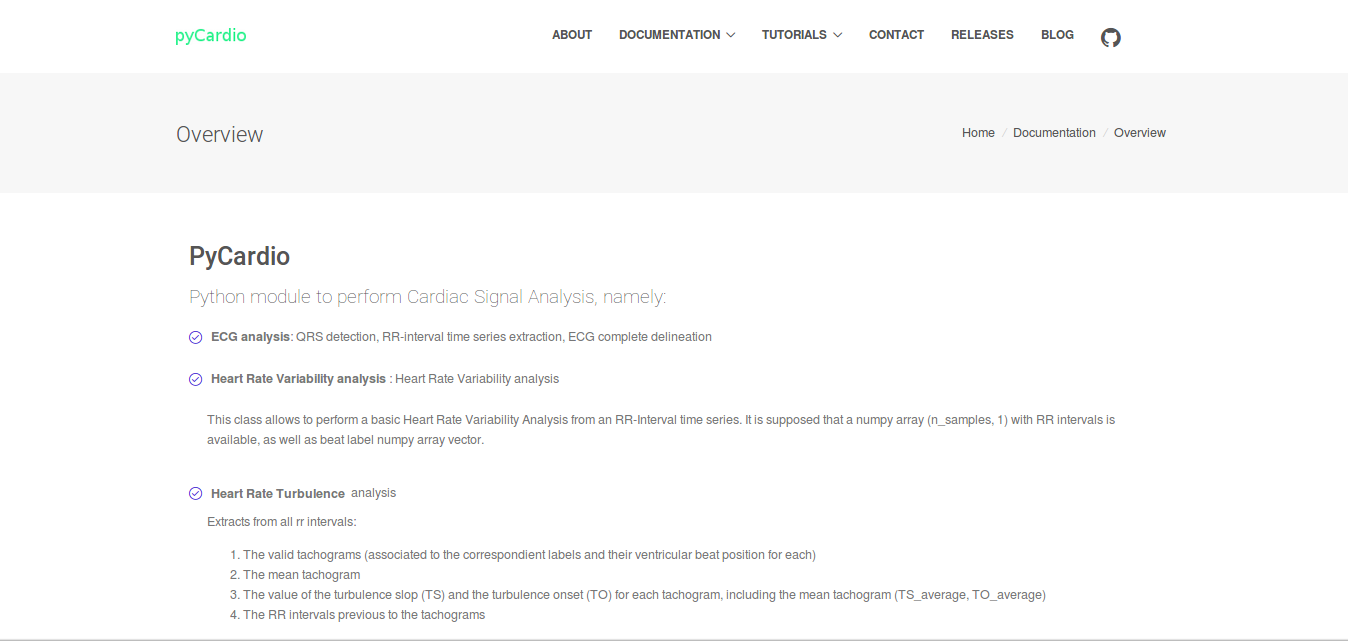
\includegraphics[width=0.5\textwidth]{img/doc_1.png}
        \label{fig:docWeb1}
    }
    \subfloat[Sección Complete Documentation]{
        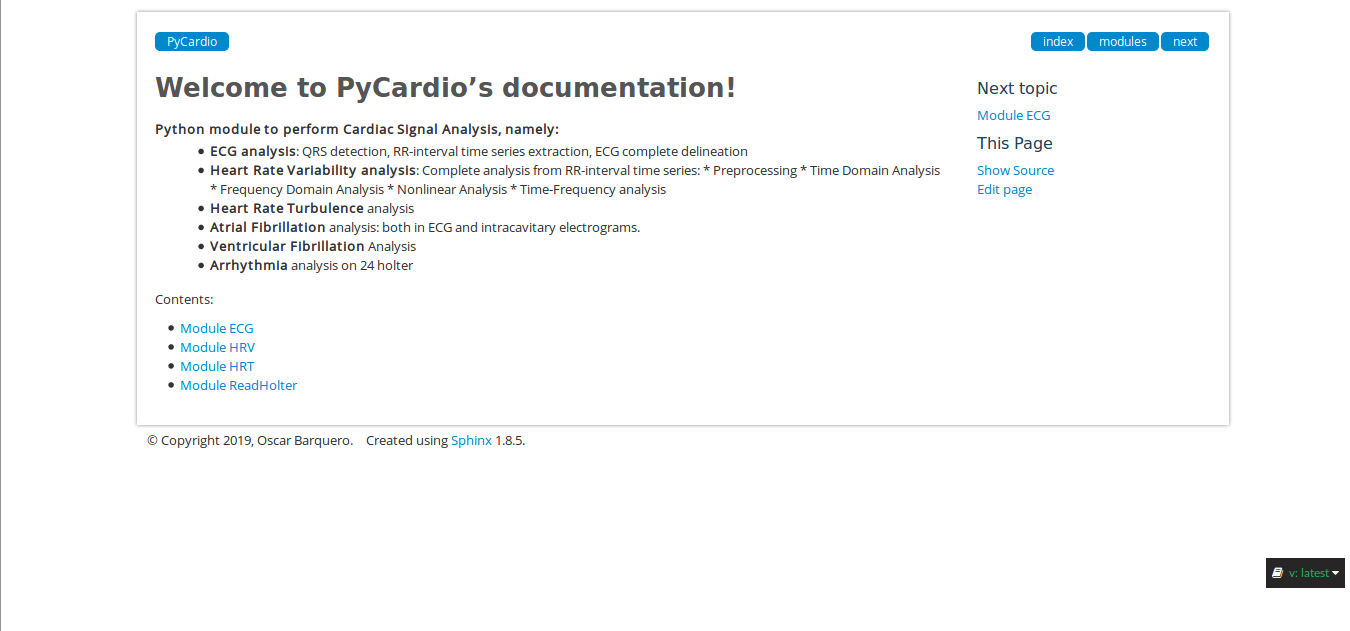
\includegraphics[width=0.5\textwidth]{img/doc_2.png}
        \label{fig:docWeb2}
    }
    \caption{Sección Documentation de la web PyCardio}
    \label{fig:docWeb}
\end{figure}


Para la implementación del contenido que se muestra en la figura \ref{fig:docWeb1} hemos usado la plantilla definida de \texttt{page.html}, por tanto, para su desarrollo lo único que ha hecho falta es escribir el contenido que esta contendrá en HTML. Como ya sabemos, la página mostrada en la figura \ref{fig:docWeb2} es la que se ha implementado en el capítulo \ref{chap:codeManagement} con la tecnología Read The Docs.


%%%%%%%%%%%%%%%%%%%%%%%%%%%%%%%%%%%%%%%%%%%%%%%%%%%%%%%%%%%%%%%%%%%%%%%%%%%%%%%%%%%%%%%%%%
%                       TUTORIALS
%%%%%%%%%%%%%%%%%%%%%%%%%%%%%%%%%%%%%%%%%%%%%%%%%%%%%%%%%%%%%%%%%%%%%%%%%%%%%%%%%%%%%%%%%%

\section{Tutorials}
\label{sec:tutoWeb}

Parte de la web centrada  tanto en dar un guión de como empezar a usar el paquete PyCardio como en mostrar un ejemplo de uso para cada módulo que compone el software. Para ello se divide en cinco apartados, uno por cada módulo y uno exclusivo para mostrar como empezar a aplicar PyCardio a nuestros desarrollos.

Antes de mostrar el contenido de este apartado es de mencionar que está incompleto debido a que el paquete sigue en fase beta y por tanto la parte de información de como usar sus módulos también. Por ello, se ha implementado el contenido de la parte que muestra como usarlo, y el tutorial del módulo HRV. 

\begin{figure}[H]
    \centering
    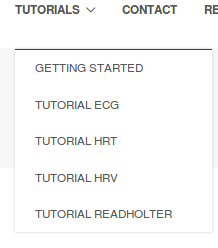
\includegraphics[width=0.5\textwidth]{img/tutorials_panel.png}
    \caption{Secciones de Tutorials }
    \label{fig:tutoWebPanel}
\end{figure}





\subsection*{Getting Started}
El contenido web de esta subsección de \textit{tutorials} centra en enseñar como instalar el paquete y como aplicarlo. Al no disponer de la información de como usar el paquete, se ha procedido a implementar una plantilla para su uso futuro cuando se disponga de mas información. En dicha plantilla podemos distinguir trozos de inserción de código, gráficas y texto. 

\begin{figure}[H]
    \centering
    \subfloat[Getting Started 1]{
        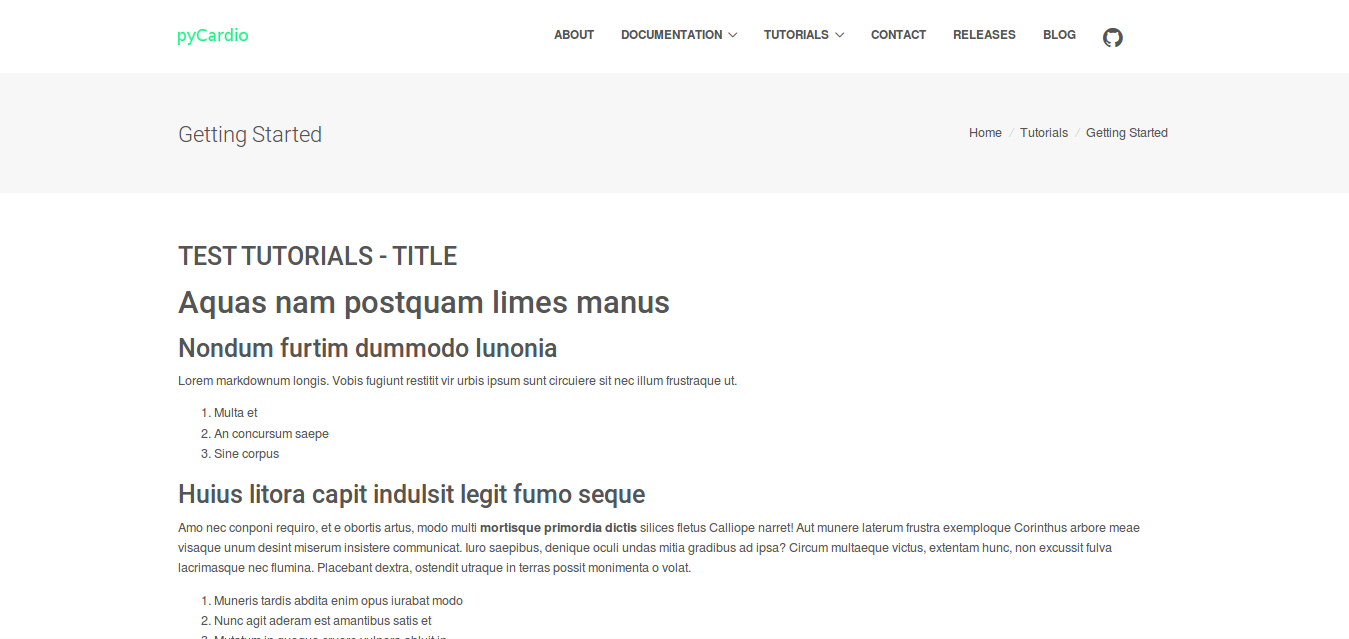
\includegraphics[width=0.3\textwidth]{img/gettin_1.png}
        \label{fig:gettinWeb1}
    }
    \subfloat[Getting Started 2]{
        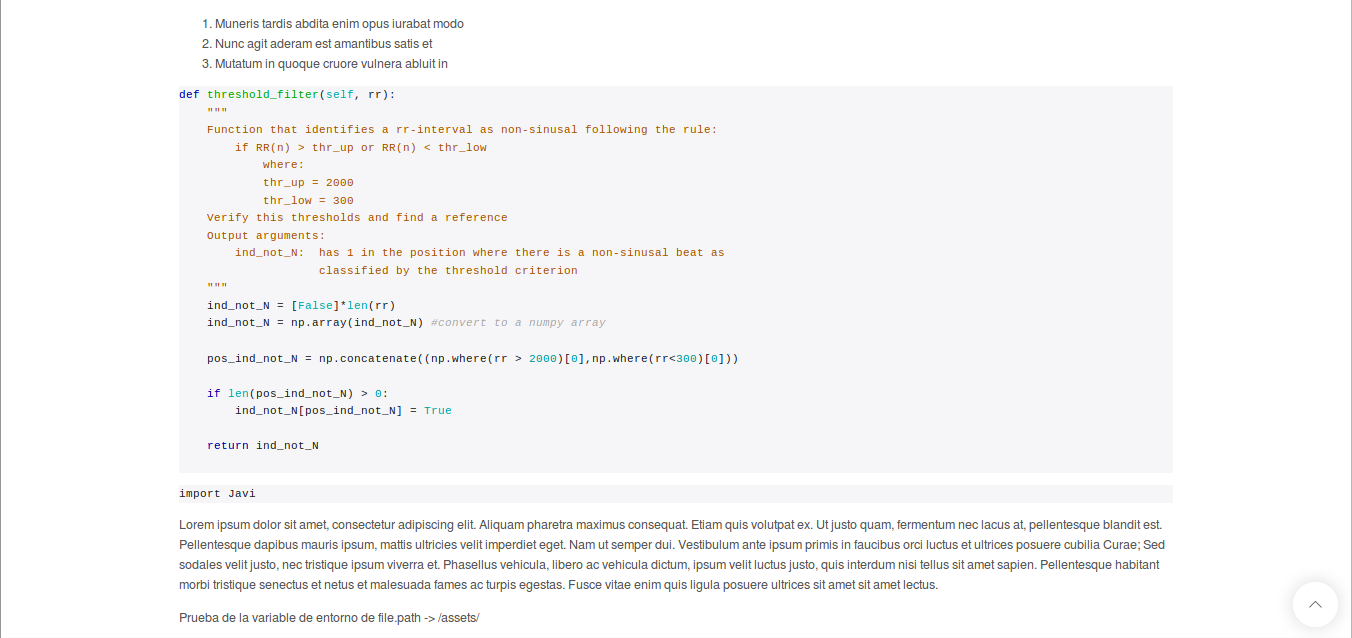
\includegraphics[width=0.3\textwidth]{img/gettin_2.png}
        \label{fig:gettinWeb2}
    }
    \subfloat[Getting Started 3]{
        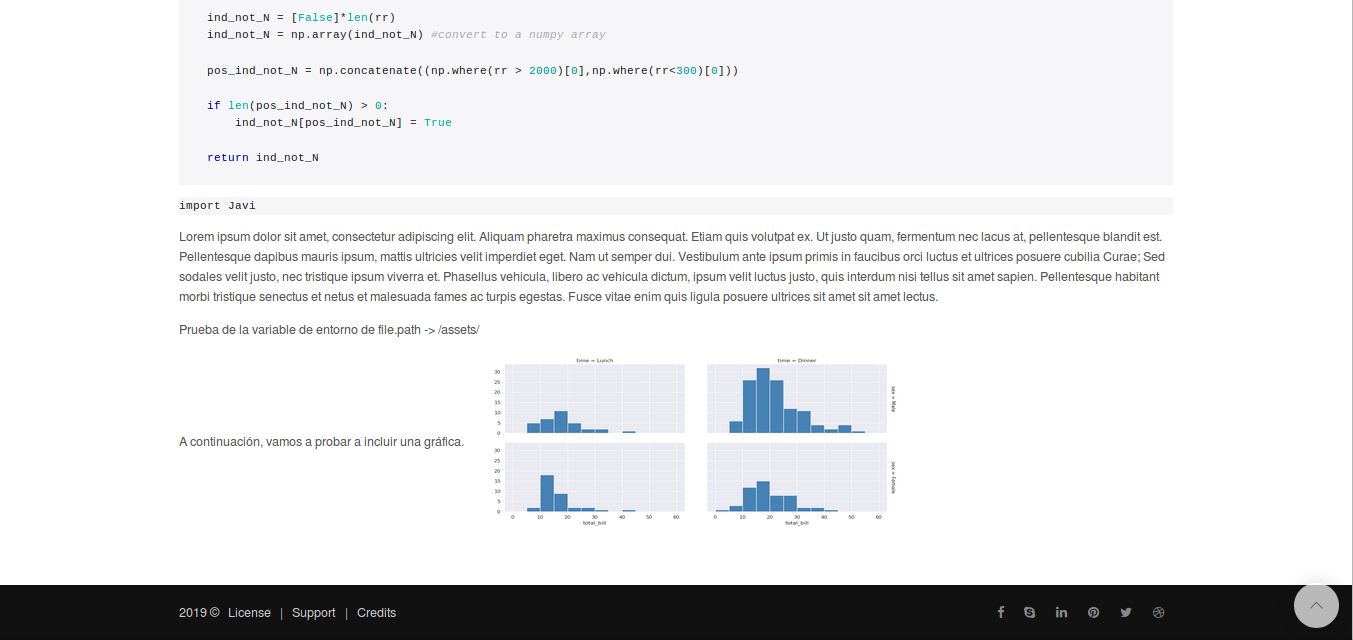
\includegraphics[width=0.3\textwidth]{img/gettin_3.png}
        \label{fig:gettinWeb3}
    }
    \caption{Subsección Getting Started de Tutorials }
    \label{fig:my_label}
\end{figure}

Su implementación a diferencia de lo demás visto hasta ahora esta escrita en MarkDown. Para ello, como venimos haciendo, en el Front Matter de nuestro fichero damos un título y referenciamos el layout que se va a usar para mostar el contenido escrito. 

\begin{lstlisting}[language=yaml,caption=getting\_started.md,label={code:gettingMark}]
  ---
layout: page
title: Getting Started
---
<!-- TUTORIALS EXAMPLE -->
<!-- TEXT -->
## TEST TUTORIALS - TITLE

# Aquas nam postquam limes manus

## Nondum furtim dummodo Iunonia

Lorem markdownum longis. Vobis fugiunt restitit vir urbis ipsum sunt circuiere
sit nec illum frustraque ut.

1. Multa et
2. An concursum saepe
3. Sine corpus

Prueba de la variable de entorno de file.path -> {{site.path_assets}}

<!-- Al necesitar reescalarla, tenemos que incluirla mediante HTML -->
<img alt="example" src="/assets/img/maps/Figure_test.png" width="500" height="200">
\end{lstlisting}

Si observamos las  últimas líneas del Listing \ref{code:gettingMark} podemos ver que también es posible escribir HTML en nuestro contenido, aunque el archivo sea de tipo MarkDown.

\subsection*{Tutorial HRV}


